\documentclass{report}
\usepackage{hyperref}
\usepackage[ngerman]{babel}
\usepackage{amsmath}
\usepackage{amsfonts}
\usepackage{amsthm}
\usepackage{tcolorbox}
\usepackage[a4paper, total={7in, 9in}]{geometry}
\usepackage[font={scriptsize,it}]{caption}
\usepackage{scrextend}
\usepackage{graphicx}
\usepackage{caption}
\usepackage{subcaption}
\usepackage[utf8]{inputenc}
\usepackage[T1]{fontenc}
\DeclareUnicodeCharacter{2212}{-}
\usepackage{verbatim}
\usepackage{tikz}

\tikzset{
  treenode/.style = {shape=rectangle, rounded corners,
                     draw, align=center,
                     top color=white, bottom color=blue!20},
  root/.style     = {treenode, font=\Large, bottom color=red!30},
  env/.style      = {treenode, font=\ttfamily\normalsize},
  dummy/.style    = {circle,draw}
}

\tikzstyle{level 1}=[level distance=3.5cm, sibling distance=3.5cm]
\tikzstyle{level 2}=[level distance=3.5cm, sibling distance=2cm]

% floating figure for column
\newenvironment{Figure}
	{\par\medskip\noindent\minipage{\linewidth}}
	{\endminipage\par\medskip}

\theoremstyle{definition}
\newtheorem{definition}{Definition}

\theoremstyle{example}
\newtheorem*{example}{Example}

\begin{document}

\begin{titlepage}
   \vspace*{\stretch{1.0}}
   \begin{center}
      \Large\textbf{eHealth exam Prep - HS20}\\
      \large\textit{Pascal Brunner - brunnpa7}
   \end{center}
   \vspace*{\stretch{2.0}}
\end{titlepage}

% Beispiel Bild
%\begin{Figure}
%   \centering
%    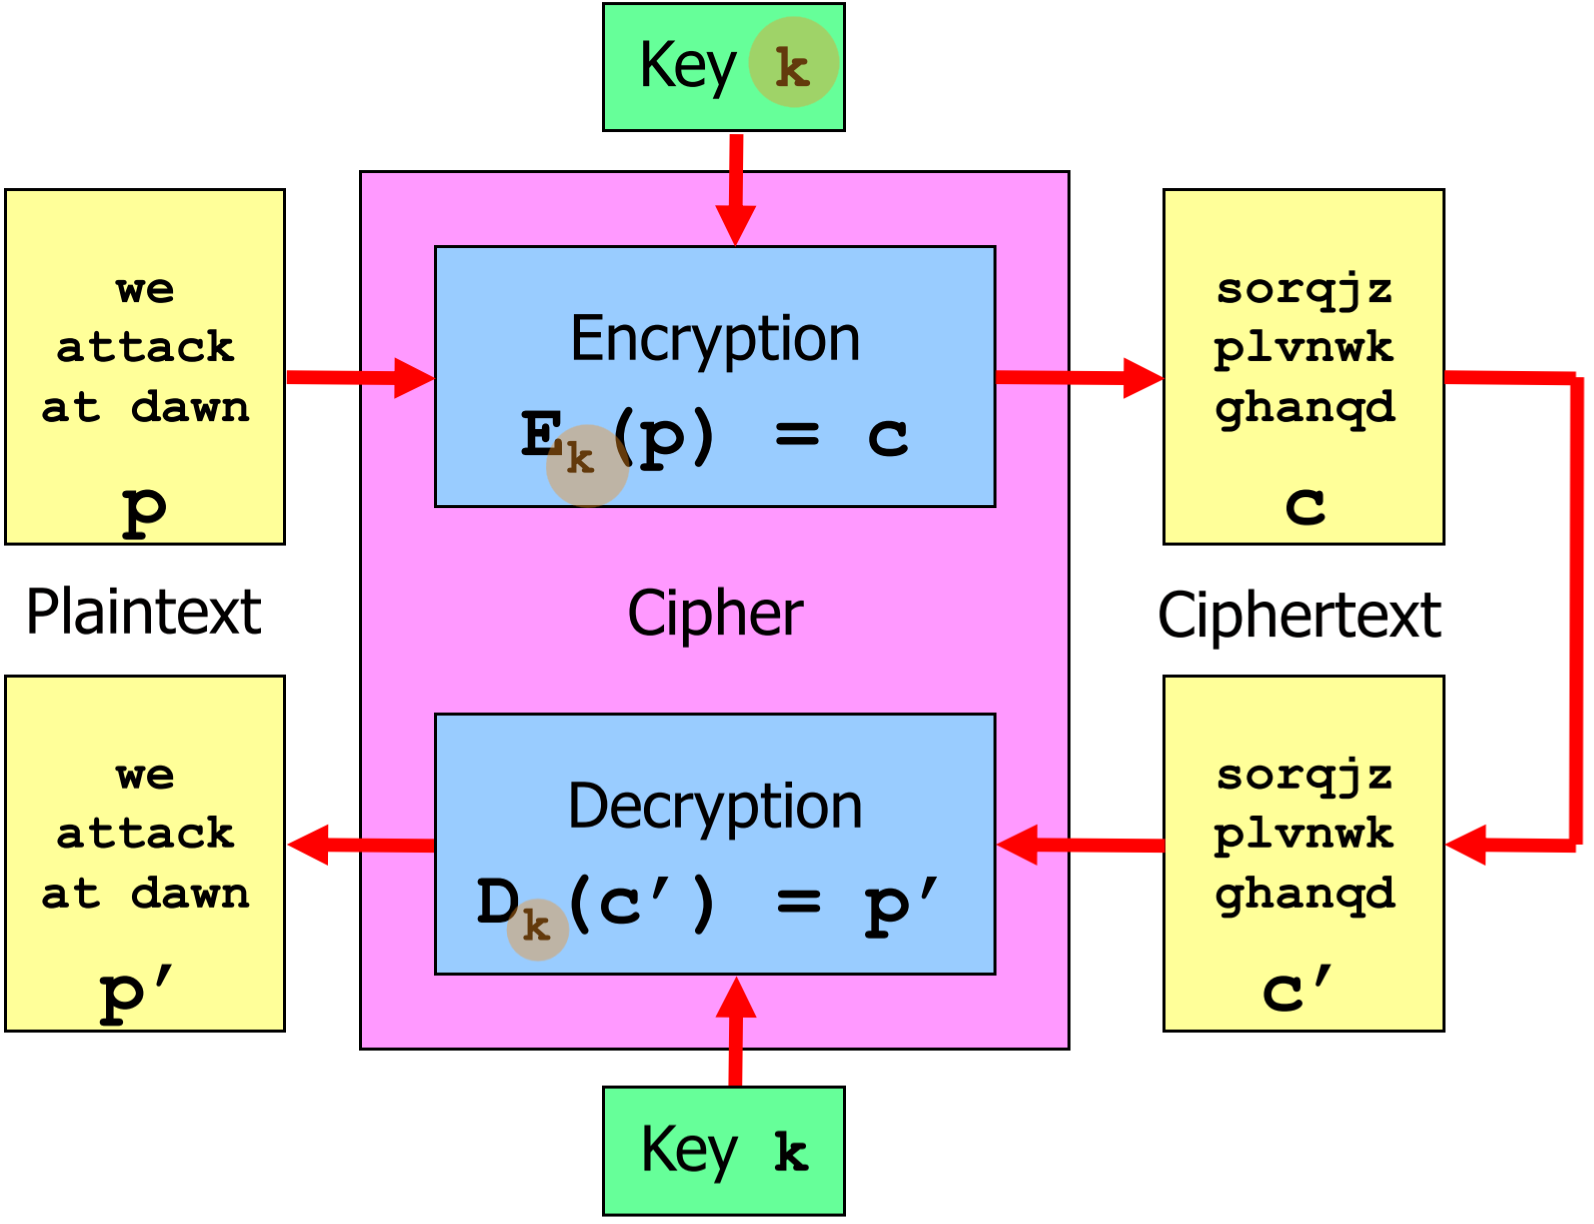
\includegraphics[width=150px]{img/BasicTerminologySecKeyCrypto.png}
%        \captionof{figure}{Basic Terminology basierend auf Secret Key Cryptography}
%        \label{fig:Basic Terminology}
%    \end{Figure}

\tableofcontents

\newpage

\chapter{Herausforderungen in eHealth Projekten}

\section{die wichtigsten Punkte}
\begin{itemize}
   \item Das Ecosystem rund um die Gesundheitsbranche (care / healthcare) ist sehr komplex
   \item sehr viele Stakeholder sind involviert (Patienten, Krankenversicherungen, Pharma Industrie, Staat, Spitex und co, Pflegearbeiter, Consultants, Lobbyisten)
   \item sehr viele kleine Organisation im Prozess
   \item Vielfältigkeit des Workflows $\rightarrow$ jeder hat sein eigens 'Kingdom', welches nicht einfach ist zu generalisieren 
   \item Unterschiedliche Motivationen und Anreize
   \item Ein Arzt hat eine Ziele wie ein Spital
   \item Höhere Qualität und bessere Effizienz resultiert nicht zwingend in bessere Resultate für den Patienten bzw. bringt nicht zwingend mehr Geld ein für den Arzt / Spital
   \subitem Der bessere Umgang bzw. das bessere Management mit chronisch Kranken Patienten kann den Anbieter sogar zusätzliches Geldkosten
   \item Auffand die Daten zu erheben / einzugeben vs. der eigentliche Mehrwert
   \item fehlender 'Netzwerkeffekt'
\end{itemize}

\begin{Figure}
   \centering
    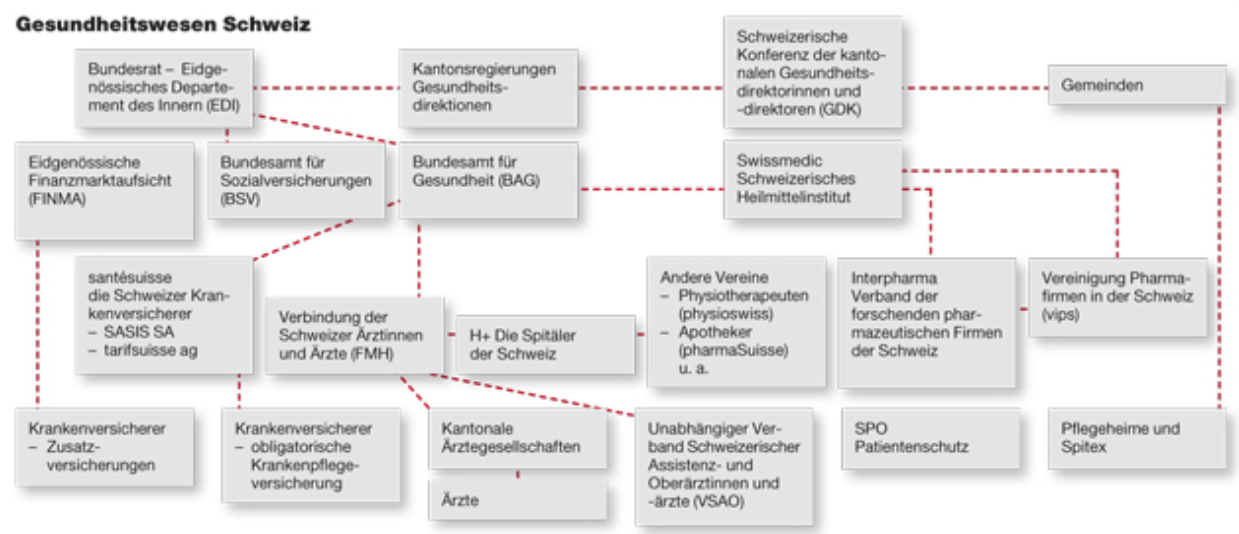
\includegraphics[width=300px]{img/swissEcosystem.png}
        \captionof{figure}{Abbildung des schweizer Ecosystem mit dem public-private-Mix}
        \label{fig:Abbildung des schweizer Ecosystem mit dem public-private-Mix}
    \end{Figure}

    \begin{itemize}
      \item \textbf{Politik}: Die Vernehmlassungen und Entscheidungen liegen häufig in der Hand der Politik. Jedoch ist die Politik eine Mischung aus verschiedenen Personen mit unterschiedlichen Zielen und Werte. Dies kann ein gefährlicher Mix sein für wichtige Entscheidungen rund um eHealth
      \item \textbf{Validierung}: Bei neuen Technologien und Decision-Support-Systemen wird das System immer dann besser, wenn neue Erkenntnisse an den Tag kommen. Doch ab wann gilt ein System als genügend gut?
      \item \textbf{Datenschutz}: Der Datenschutz erreicht eine neue Dimension, die es sowohl national, wie aber auch international zu regeln gilt. Wie wird sichergestellt, dass die korrekten Personen Zugriff auf die Daten haben, jedoch gleichzeitig sichergestellt wird, dass für Unbefugte die Daten nicht abgreifbar sind. So lange man sich innerhalb eines Spitals befindet lassen sich diese Anforderungen gut umsetzen, nun kommt aber der Faktor dazu, dass EHR plötzlich von zuhause aus zugreifbar sind. Wie kann man dann gewährleisten, dass der Datenschutz auch gewährleistet ist.
      \item \textbf{Datenintegrität}: Die Daten müssen nicht zu einem bestimmten Zeitpunkt zugreifbar sein, sondern zu jedem Zeitpunkt muss die Integrität gewährleistet werden. 
      \item \textbf{Identifikation}: Neben der Integrität muss die Eindeutigkeit gewährleistet werden, wie kann man den einzelnen Patienten national oder international eine eindeutige Identifikation ausweisen?
      \item \textbf{Zuverlässigkeit}: Wenn beispielsweise Level 7 erreicht wird, so hat das Spital kein einziges Blatt-Papier mehr im Einsatz, sondern alles digital. Dadurch wächst jedoch auch der Anspruch an Zuverlässigkeit. Was passiert wenn einmal das Internet oder der Strom aussteigt? 
      \item \textbf{Angriffsfläche}: Je mehr Daten und Informationen und vor allem die Abhängigkeit auf das Digitale abgewälzt wird, desto grösser wird die Angriffsfläche eines Spitals / Gesundheitssystem und dadurch haben auch immer mehr Personen Interesse an einem Angriff auf das Spital (Hacker)
      \item \textbf{Datenaustausch}: Wie kann der Datenaustausch zwischen zwei Insituation (Spital - Spital, Patient - Spital, Patient - Angehörige etc.) sicher gestaltet werden? 
   \end{itemize}

\section{Ausblick / Vision}
\begin{itemize}
   \item Verbesserungen der Qualität der Pflege, der Wissenschaft und der medizinalen Ausbildung
   \item Mittelfristig:
   \subitem Digitale Transformation: ICT-Tools und Prozesse
   \subitem elektronische Gesundheits-Record (EHR) und Datengetriebene Services
   \subitem Digitale Integration, semantische Interoperabilität, mHealth
   \item Langfristig: 
   \subitem individuelle, personalisierte Medizin (genomics data)
   \subitem Querschnittliche Verwendung der EHR-Daten, Daten-Analyse und Big Data
   \subitem Knowledge Management, Medizinische Entscheidungs-Support-Systeme (DSS) und Deep Learning / KI 
\end{itemize}

\chapter{rechtliche und ethische Fragen}

\begin{itemize}
   \item \textbf{Einschränkung durch Technologie}: Die Interoperabilität ist eine zwingende Bedingung. Andernfalls kann das Personal durch die Technologie beeinträchtigt werden und ihrer Verpflichtung nicht mehr nachkommen. Wer ist dann bspw. für das Versterben eines Patienten verantwortlich?
   \item \textbf{Haftung}: Wer haftet, wenn ein System ausfällt und dadurch eine Behandlung nicht durchgeführt werden kann. System $\rightarrow$ WLAN, CIS, Geräte etc.
   \item \textbf{Kostenverteilung}: Wer hat die anfallenden Kosten für das eHealth-Ecosystem zu übernehmen? Staat, Krankenkasse, Patient?
   \item \textbf{Langfristige Planung}: Wie kann aus ethischer Sicht gewährleistet werden, dass das einführende (Eco-)System langfristig robust eingesetzt werden kann und laufend erweitert und ergänzt wird? 
   \item \textbf{Datenschutz:} Sensible Daten, wer darf was, wann sehen? 
   \item \textbf{Datensicherheit:} Unter welchen Bedingungen dürfen die Daten gespeichert werden und welche Einschränkeun (bspw. geografie)
   \item \textbf{Forschung:} Auf welche Daten darf die Forschung zugreifen? In welcher Form müssen die Daten bearbeitet / anonymisiert werden für eine Forschung.
   \item \textbf{Bias:} Rücksichtnahme auf die unterschiedlichen Menschenherkunft (Hautfarbe, Merkmale bspw. asiatische Augen)
\end{itemize}


\chapter{Hauptkomponente in einem Clinical Information System - L02}
CIS $\rightarrow$ Clinical Information System\\
Das CIS ist ein Bestandteil eines Healthcare Information System (HIS). Zu einem HIS gehört neben dem CIS noch ein Administrative-Information-System.\\

\textbf{Vorteile eines integrierten CIS}
\begin{itemize}
   \item Verbesserung des Informationszugangs
   \item bessere Dokumentation
   \item Erhöht die Qualität der Pflege und reduziert die Medikations-Fehler 
   \subitem Elimiert Transkription Fehler
   \subitem Beschleunigt Behandlung
   \subitem genauere, kompletere Bestellungen
   \item Verbessert die Produktivität und Kommunikation zwischen dem Pflegepersonal
   \item Tracking Möglichkeiten
   \item verbesserte Einhaltung von Vorschriften 
\end{itemize}

\section{Teile eines CIS}
CIS hat mehrere Hauptbestandteile, welche nachfolgend erläutert werden.

\subsection{Nursing Information System / Krankenpflege}
\begin{itemize}
   \item Unterstützt die Tätigkeit des Pflegepersonals
   \item Unterstützt die Dokumentation 
   \item Ansehen / Aktualisieren der Patienten-Daten / Patienten-Zustand
   \item Zugriff auf die aktuelle Medikation 
   \item Verfahrensrichtlinien Datenbanken
   \item Stellt die Qualität der Pflege sicher
   \item \textbf{Ziele für Verbesserung}
   \subitem Dokumentation / Zugriff zu Informationen
   \subitem Produktivität und Kommunikation
   \subitem Einhaltung gesetzlicher Vorschriften
\end{itemize}

\subsection{Monitoring Systems / Überwachung}
\begin{itemize}
   \item Überwachung der Vitalität des Patienten, sowie weitere Informationen
   \item Alarm-System, falls ein Wert einen Schwellwert erreicht
   \item Echtzeit Überwachung über die Konditionen eines Patienten
   \item Automatische Datenübertragung ins CIS
\end{itemize}

\subsection{Order Entry Systems / Bestellungseingabe}
Ein Computerized Physician Order Entry (CPOE) nimmt ärztliche Anordnungen elektronisch und ersetzt damit handschriftliche oder mündliche Anordnungen. Bietet auch Entscheidungshilfe bei der Bestellung (doppelte Tests, Wechselwirkungen zwischen Medikamenten, Allergien usw.). Es kann dem Arzt auch die Kosten für das Medikament anzeigen.\\
\textbf{Wichtig:} Ungefähr die Hälfte der Medikationsfehler treten während des Bestellvorgangs (CPOE) auf, aber auch bei der Abgabe, Verabreichung und Überwachung von Medikamenten treten Fehler auf.
\begin{itemize}
   \item Direkte Eingabe von Anordnungen für Medikamente und Behandlungen durch den
   \subitem Behandelten Arzt 
   \subitem Krankenschwester
   \subitem Pharmakologe
   \subitem Physiotherapeutin
   \item Online-Aufträge an die entsprechenden Bereiche weiterleiten
   \subitem Apotheke
   \subitem Labor
   \subitem Radiology
   \subitem etc. 
\end{itemize}

\subsection{Laboratory System}
\begin{itemize}
   \item Verwaltung der Labor-Teste (Bluttest oder Körpergewebe)
   \item Informiert / alarmiert wenn Testresultate eingetroffen sind oder einen kritischen Wert haben
   \item Sendet Resultate ins CIS
   \item Akzeptiert Eingaben eines Gerätes am Krankenbett
   \item Etiketten für die Probenentnahme generieren
   \item Anwendung von Regeln für das Beauftragen von erneuten Tests
   \item Problemerkennung (Umschlagsdauer, Duplikate, Fehler)
   \item Standard-Codenames: LOINC
   \subitem Logical Observation Identifiers Names and Codes (LOINC)
   \subitem Code-namen und IDs für den elektronisches Austausch von klinischen Informationen (bspw. Laborteste)  
\end{itemize}

\subsection{Radiology System}
\begin{itemize}
   \item Radiologie = Röntgenstation
   \item Ermöglicht direkte Auftragseingabe oder akzeptiert Aufträge aus anderen Systemen
   \item Einplanen von Diagnosen-Tests
   \item Erstellt Kundenauftrag
   \item Abschriften / Transkription der Ergebnisse zulassen
   \item Stellt ein Bildarchiv und dessen Übertragung zur Verfügung
   \item Erstellt die Abrechnung sobald eine Behandlung abgeschlossen ist
   \item \textbf{Standard: PACS}
   \subitem Picture Archiving and Communication System (PACS)
   \item Transferiert X-Ray/CT/MRI-Bilder zu PACS
   \item verlinkt die Bilder zum Patientendossier im CIS
   \item Bietet Analysemöglichkeiten der Bilder
   \item Zugang zu den Resultaten: Suchen, Anzeige, Annotieren
\end{itemize}

\subsection{Pharmacy System}

\begin{itemize}
   \item \textbf{eMedication / ePrescription}
   \item Kontrollen im Bestell- und Verabreichungsprozess anhand von evidenzbasierten Richtlinien durchführen
   \item Administration durch Barcode und RFID Medikation
   \item Dosierungsanlage (Roboter)
   \item Verwendung und Interaktion der CIS Informationen (Laborresultate, Allergien etc.)
   \item Tracking der Medikation (Verwendung, Kosten und Abrechnung)
   \item \textbf{Electronic Medication Administration Record (eMar)}
   \item Bereitstellung eines langfristigen Verordnungsdatensatzes
   \item Überprüfung der Formalitäten, Compliance und Erstattungen
   \item Warnungen über Wechselwirkungen von Medikamenten
   \item Abwicklung über das Telefon für die Nachfüllung entfällt
   \item Lesefehler bei der Apotheke entfällt
   \item \textbf{Bar-Code-enabled Point of Care (BPOC)}
   \subitem Durch Barcode bei den Medikamenten und am Handgelenk des Patienten wird sichergestellt $\rightarrow$ korrekte/r Patient, Medikamentation, Dosierung, Zeit, Ablauf
   \subitem Alternative Verwendung durch RFID
\end{itemize}


\subsection{weitere Hilfssysteme}
\begin{itemize}
   \item Praxisverwaltungssystem für Ärzte
   \subitem Erfassung von demografischen und Versicherungsdaten, Terminplanung, Abrechnung, Ergebnisverfolgung und Berichtsfunktion
   \subitem Kann mit der elektronischen Patientenakte des Krankenhauses verbunden werden oder separate Patientenakten führen 
   \item Home Healthcare Management System
   \subitem Kommunikation mit dem Spital inkl. Austausch von Daten
   \subitem Telemedizin Support
   \subitem Unterstützung bei übermässig vielen Dokumentationen
   \subitem Verbesserung des Zahlungsprozesses
   \item Ambulanz
\end{itemize}

\chapter{Aktuelle Situation in der Schweiz für das elektronische Patientendossier - L03 / L03a}

\section{Schweiz}

Gesetz seit 15.April.2017 für EHR $\rightarrow$ Spitäler (ab 2. Quartal 2020) und Pflegeheime (ab 2022) müssen ihre Daten dort ablegen.\\
Die Spitäler hatten die Frist, die EHR im 2. Quartal 2020 einzuführen - dies war aber aufgrund von Verzögerungen durch die Zertifizierungsstelle nicht möglich (neuestes Factsheet (Juli 2020). Die Einführung erfolgt iterativ, d.h. von Kanton zu Kanton. Die Einführung erfolgt auch dezentral, durch die verschiedenen Zertifizierungsstellen.\\
Es ist geplant, dass die Einführung bis zum Ende des ersten Quartals 2021 in jedem Kanton abgeschlossen sein wird. Ein detaillierter Rollout-Plan kann hier eingesehen werden.\\

\subsection{Ausführlichere Variante}

Seit dem 15. April 2017 gibt es in der Schweiz das neue Gesetz zur EHR. Spitäler müssen an der EHR teilnehmen und die Gesundheitsinformationen in der EHR ablegen, ebenso Pflegeheime ab 2022. Für alle anderen Behandelnden, wie Hausärzte, Apotheken oder Spitexdienste, ist die Teilnahme freiwillig. 
Die EHR ist auch für die Bürgerinnen und Bürger freiwillig. Die Spitäler hatten die Frist, die EHR im 2. Quartal 2020 einzuführen - dies war aber aufgrund von Verzögerungen durch die Zertifizierungsstelle nicht möglich (neuestes Factsheet (Juli 2020). Die Einführung erfolgt iterativ, 
d.h. von Kanton zu Kanton. Die Einführung erfolgt auch dezentral, durch die verschiedenen Zertifizierungsstellen. Es ist geplant, dass die Einführung bis zum Ende des ersten Quartals 2021 in jedem Kanton abgeschlossen sein wird. Ein detaillierter Rollout-Plan kann hier eingesehen werden.

Auch Deutschland strebt eine Einführung bis Januar 2021 an. Allerdings sind hier die Krankenkassen die treibende Kraft bzw. die Behörde, die zur Einführung verpflichtet ist. Aber auch in Deutschland ist die Nutzung des Systems für die Bürger freiwillig. 

Anders ist es bereits weiter nördlich - in Dänemark - wo jeder Einwohner eine sogenannte nemID erhalten hat. Diese ID ermöglicht es jedem Bürger, sich eindeutig zu identifizieren, um z.B. auf offizielle Dokumente zuzugreifen. Dabei kann nicht nur auf die wichtigsten amtlichen Dokumente zugegriffen werden, sondern auch die elektronische Patientenakte verwaltet werden. 
So kann der Bürger Familienmitgliedern Zugang gewähren, Organspenden können organisiert und manuelle Informationen wie der Blutdruck direkt eingegeben werden.

\subsection{Zertifizierungsstellen pro Kanton}
\begin{itemize}
   \item \href{https://www.cara.ch/}{cara.} $\rightarrow$ FR, GE, JU, VD, VS
   \item \href{https://hesav.ch/dossier-sante/}{dossier santé} $\rightarrow$ NE
   \item \href{https://www.xsana.ch/bevoelkerung#benefits}{xsana} $\rightarrow$ BE, BL, BS, LU, NW, OW, SG, SH, SO, SZ, TG, UR, ZG, ZH
   \item \href{https://www.mein-emedo.ch/}{emedo} $\rightarrow$ AG 
   \item \href{https://www.ehti.ch/}{e-Health Ticino} $\rightarrow$ TI
   \item \href{https://esanita.ch/}{eSanita} $\rightarrow$ AI, AR, GL, GR, SG
   \item \href{https://www.abilis.ch/de}{abilis} $\rightarrow$ national, Switzerland
\end{itemize}

\subsection{Anbieter}
\begin{itemize}
   \item evita von Swisscom
   \item Lösung von der Post
\end{itemize}

\subsection{Deutschland}
Auch Deutschland strebt eine Einführung bis Januar 2021 an. Allerdings sind hier die Krankenkassen die treibende Kraft bzw. die Behörde, die zur Einführung verpflichtet sind. Aber auch in Deutschland ist die Nutzung des Systems für die Bürger freiwillig.

\subsection{Nordeuropa}
Anders ist es bereits weiter nördlich - in Dänemark - wo jeder Einwohner eine sogenannte nemID erhalten hat. Diese ID ermöglicht es jedem Bürger, sich eindeutig zu identifizieren, um z.B. auf offizielle Dokumente zuzugreifen. Dabei kann nicht nur auf die wichtigsten amtlichen Dokumente zugegriffen werden, sondern auch die elektronische Patientenakte verwaltet werden. So kann der Bürger anderen Familienmitgliedern den Zugang gewähren, Organspenden können organisiert und manuelle Informationen, wie der Blutdruck direkt eingegeben werden

\chapter{FHIR queries / code - L05}

\section{HL7 v2.n}
Alter Standard von HL7, am weitestens verbreitet (Name-Value Pair)
\begin{itemize}
   \item Gut innerhalb einer Organisation
   \item Funktioniert via Anfragen (Request, Respond)
\end{itemize}

\section{HL7 FHIR STU}
Fast Healthcare Interoperability Reosurce
\begin{itemize}
   \item Biete ca. 80\% (aber erweiterbar)
   \item Gratis
   \item RESTful API (XML, JSON, HTTP)
\end{itemize}

\section{Operationen}

\textbf{Instance}
\begin{itemize}
   \item \textit{Read:} \textbf{GET} [base]/Patient/100
   \item \textit{Update:} \textbf{PUT} [base]/Patient/100
   \item \textit{Delete:} \textbf{DELETE} [base]/Patient/100
   \item \textit{History:} \textbf{GET} [base]/Patient/100/\_history
   \item \textit{Version-read:} \textbf{GET} [base]/Patient/100/\_history/\{vid\}
\end{itemize}

\textbf{Type}
\begin{itemize}
   \item \textit{Create:} \textbf{POST} [base]/Patient
   \item \textit{Search:} \textbf{GET} [base]/Patient?name=eve
   \item \textit{History:} \textbf{GET} [base]/Patient/\_history
   \item \textit{Read:} \textbf{POST} [base]/Patient/\{id\}/\$validate
\end{itemize}

\textbf{System}
\begin{itemize}
   \item \textit{Conformance:} \textbf{GET} [base]/metadata
   \item Transaction \textbf{POST} bundle to root
   \item \textit{History:} \textbf{GET} [base]/\_history
\end{itemize}

\textbf{Bindings}
\begin{itemize}
   \item \textit{Required:} \textbf{!} $\rightarrow$ must come from set
   \item \textit{Extensible:} \textbf{+} $\rightarrow$ May use alternate if have to
   \item \textit{Preferred:} \textbf{?} $\rightarrow$ don't have to, but should
   \item \textit{Example:} \textbf{??} $\rightarrow$ set isn't specified
\end{itemize}

\textbf{Und / Oder}
\begin{itemize}
   \item \textit{Und:} \textbf{\&}
   \item \textit{Oder:} \textbf{,}
   \item $\Rightarrow$ fhir/Patient/\_search?birthdate=1972-11-30\textbf{\&}language=nl\textbf{,}fr
\end{itemize}

\textbf{Vergleichsoperatoren}
\begin{itemize}
   \item \textit{equals:} \textbf{eq}
   \item \textit{not equals:} \textbf{ne}
   \item \textit{greater than:} \textbf{gt}
   \item \textit{less than:} \textbf{lt}
   \item \textit{greater equals:} \textbf{ge}
   \item \textit{less equals:} \textbf{le}
   \item \textit{starts after:} \textbf{sa}
   \item \textit{ends before:} \textbf{eb}
   \item \textit{apporximately:} \textbf{ap}
\end{itemize}

\section{Resource URL}
\begin{Figure}
   \centering
   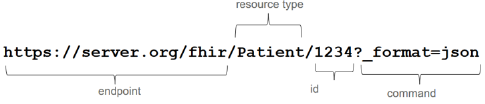
\includegraphics[width=150px]{img/FHIRResourceURL.png}
      \captionof{figure}{Zusammensetzung Resource URL in FHIR}
      \label{fig:Zusammensetzung Resource URL in FHIR}
\end{Figure}

\section{Suche URL}
\begin{Figure}
   \centering
   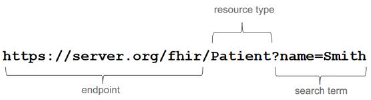
\includegraphics[width=150px]{img/FHIRSucheURL.png}
      \captionof{figure}{Zusammensetzung Suche URL in FHIR}
      \label{fig:Zusammensetzung Suche URL in FHIR}
\end{Figure}

\section{Beispiele}

\begin{Figure}
   \centering
   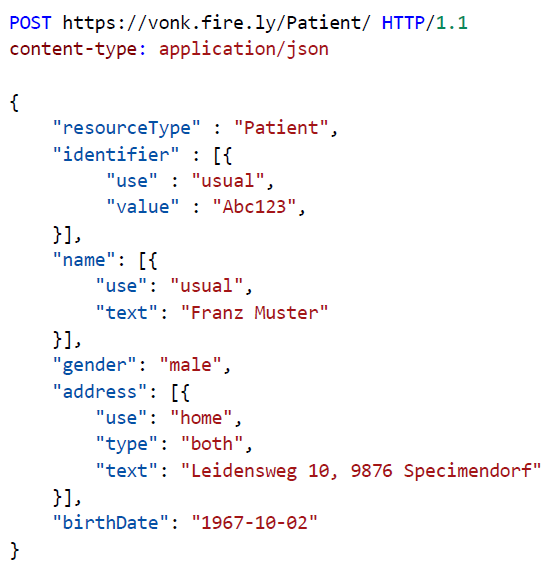
\includegraphics[width=150px]{img/FHIRCreateResource.png}
      \captionof{figure}{Beispiel Resource erstellen}
      \label{fig:Beispiel Resource erstellen}
\end{Figure}

\begin{Figure}
   \centering
   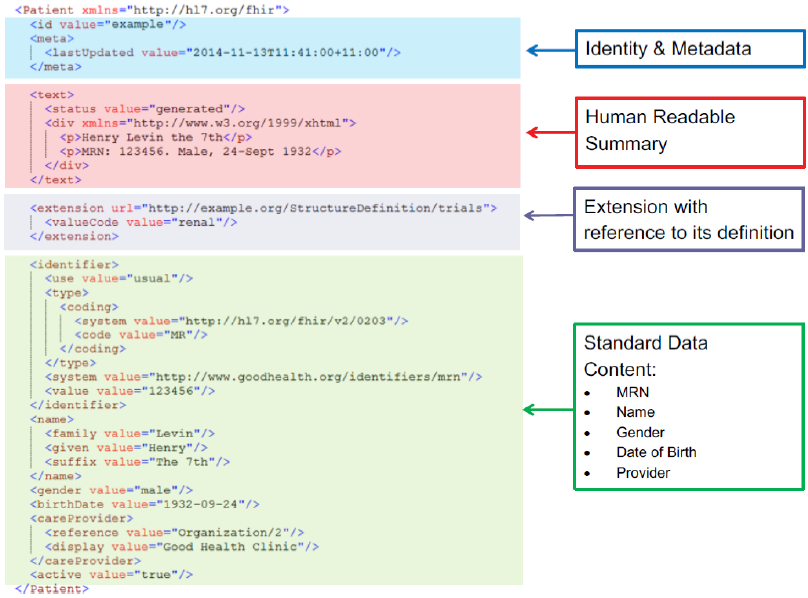
\includegraphics[width=150px]{img/FHIRResponse.png}
      \captionof{figure}{Beispiel FHIR Response}
      \label{fig:Beispiel FHIR Response}
\end{Figure}

\chapter{Herausforderungen medical decision support system - L07}

\section{Ausgangslage}
Ein medical decision support braucht für die Entscheidung das akkumulierte Wissen aus den unterschiedlichsten Gebieten. Vergleichebare Werte müssen vorliegen um ein spezifisches Problem, Resultat oder Diagnose zu ermitteln.\\
Sehr häufig müssen Entscheidungen mit limitiertem Wissen, nicht-kompleten Informationen innerhalb einer sehr kurzen Frist gefällt werden.\\
Während der Behandlung tauchen viele Fragen auf, heute bereichert man sein Wissen
\begin{itemize}
   \item Arbeitskollegen
   \item Internet-Ressourcen
   \item Medizinische Guidelines
   \item Medizinische Handbücher
   \item Suche in bibliografische Retrieval-Systeme (PubMed)
\end{itemize}
Diese Quellen stellen Informationen zur Verfügung, helfen jedoch nicht diese anzuwenden. $\rightarrow$ viele Fragen bleiben unbeantwortet

\section{Herausforderung im medizinischen Wissen}
\begin{itemize}
   \item Das Wissen multipliziert sich schneller und schneller
   \subitem Medizinische Literatur verdoppelt sich alle 19 Jahre
   \subitem Genexpressionsanalysen verdoppeln sich alle 8 Monate
   \item Fehler / Irren ist menschlich
   \subitem Ungenaue Diagnosen, falsche Behandlungen, falsche Medikation
   \item Wissens-Zugriff und Entscheidungsunterstützung zum Zeitpunkt der Behandlung
   \subitem Repräsentation und Verwaltung von medizinischem Wissen
   \subitem Integration von weiteren Tools im Prozess
   \item Forderung nach Veränderung zur Steigerung von Qualität und Sicherheit
   \item Von reaktivem Verhalten zu proaktivem
   \item Von Klinik-zentriert zu Patienten-zentriert
   \item Von episodischen Antworten zu durchgehende Gesundheits-Monitoring
\end{itemize}


\chapter{Begriffe in medical imaging und human body visualization - L08 / L09}
Basis Zusammenfassung willilu1

\section{klinische Fragestellungen}
\begin{itemize}
   \item \textbf{Anatomie}: Wo liegen Läsionen, innere Blutungen etc.
   \item \textbf{Physiologie/Pathophysiologie}: Energieverbrauch, Blutdruck etc.
   \subitem Lokalisation bei Operationen, Behandlungsplanung, Screening
   \subitem Röntgen, Nuklear-Medizin, Ultraschall, MRI (Nicht ionisiert) 
\end{itemize}

\section{Radiaktiver Zerfall}

\begin{equation}
   \frac{dA}{dt} = - \lambda A
\end{equation}
Wobei A = Aktvität [Bq]

\begin{equation}
   A(t) = A_0 * e^{-(Ke+\lambda)t}
\end{equation}
Wobei Ke = Körperaufnahme

\section{Verfahren}
Es gibt unterschiedliche Verfahren, welche unterschiedliche Resultate liefert (Gewebe sichtbar, Knochensichtbar etc.)
\subsection{Positron Emission Tomography (PET)}
Bei diesem Prozess werden Positron 'geschossen'. Beim Aufschlag auf ein Elektron entsteht eine Strahlung (Anti-Teilchen-Fusion). Diese Strahlung wird verwendet um eine Aufzeichnung durchzuführen. Bei PET sind die Knochen nicht sichtbar.

\subsection{Magentic Resonance Imaging (MRI)}
Ein starker Magnet wird auf den Körper gerichtet, die Wasserstoffe innerhalb des Körpers richten sich aus. Durch das starke Vorkommen von Wasser im Körper, vor allem im Gewebe lassen sich je nach gradueller Strahlung das Bild erkennen. So lässt sich auch ein unterschiedlicher Fokus des Bildes stellen.

\subsection{Sono / Ultra Sound}
Ultraschall wird für die Untersuchung von weichem Gewebe verwendet (keine Knochen). Wobei mit 1-20 MHz ausgestrahlt wird und die Antwort verarbeitet bzw. analysiert.

\subsection{Röntgen / XRay}
Dies wird mit sogenannter Bremsstrahlung durchgeführt, diese haben einen starken Elektronenfluss von Kathode (Minuspol) auf harte Anode (Pluspol). Dabei wandelt ein Detektor die Strahlung elektrische Landung um. Diese Strahlung ist aber sehr \textbf{gefährlich}, da eine hohe Dosis zu einem Zelltod (an der betroffenen Stelle) führen kann.\\
Als Konsequenz daraus kann Haarausfall, Verbrennung bis hin zum Tod führen. \\
Ein Vorteil dieses Verfahrens ist, dass zwischen Knochen, Muskeln, Fett und Luft unterschieden werden kann. 

\subsection{Computer Tomography (CT)}
Mittels CT lassen sich 2-/3-/4-D Aufnahme tätigen. 

\begin{Figure}
   \centering
    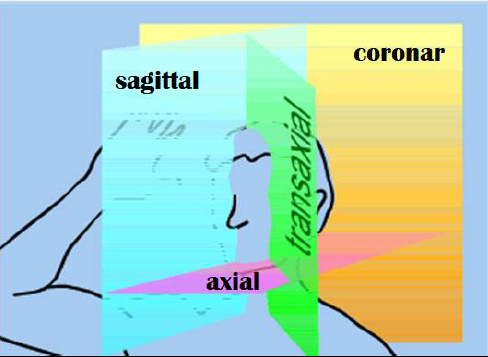
\includegraphics[width=150px]{img/CT.png}
        \captionof{figure}{Abbildung der unterschiedlichen Achsen im CT-Verfahren}
        \label{fig:Abbildung der unterschiedlichen Achsen im CT-Verfahren}
    \end{Figure}

Diese Messung passiert mit der sogenannten Hounsfield-Unit. Wobei Hounsfield [HU] ein definierter Grauwert im Vergleich zu Wasser ist. Durch unterschiedliche HU-Werte lassen sich unterschiedliche Gewebestrukturen oder Knochen in einem Bild abbilden.

\begin{equation}
   HU = \frac{\mu_x - \mu_{Wasser}}{\mu_{Wasser}} * 1000
\end{equation}

\begin{Figure}
   \centering
    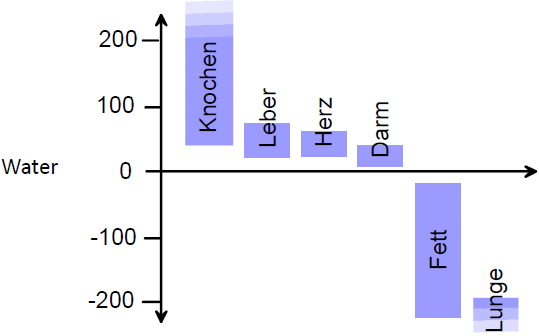
\includegraphics[width=150px]{img/Hounsfield.png}
        \captionof{figure}{Beispielmessgroessen durch Messung mit HU}
        \label{fig:Beispielmessgroessen durch Messung mit HU}
    \end{Figure}

\begin{Figure}
   \centering
   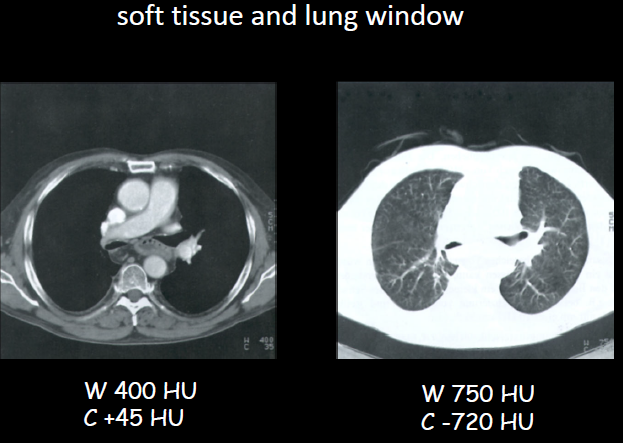
\includegraphics[width=150px]{img/HUImages.png}
      \captionof{figure}{Beispielbilder unterschiedlicher HU}
      \label{fig:Beispielbilder unterschiedlicher HU}
\end{Figure}

\section{Weitere Standards / Informationen}
Die Bilder werden mit dem speziellen Bildformat \textbf{DICOM} (Digital Imaging Communication in Medicine) abgespeichert. Dabei werden im Header Patienten- und Scanning-Daten hinzugefügt, des Weiteren findet man Informationen zur Orientierung und Grösse.\\
\textbf{Voxel}: Ist ein wichtiger Begriff beim Rendern von 3D Bildern. Dies ist die identische Grösse zu Pixel (einfach 3D) und definiert somit den Ort im Raum auf der x,y,z-Achse\\
Dabei kann man unteranderem \textbf{DVR} oder \textbf{MIP} als Verarbeitungsprozess verwenden.


\chapter{SPARQL - L10 / L11}
SPARQL ist eine Art Abfragesprache, welche jeweils in einem RDP-Triple auftritt. $\rightarrow$ Subject, Predicate, Object $\Rightarrow$ Bspw: Bob 'is interested in' Mona Lisa

\section{Operatoren}

\begin{itemize}
   \item \textit{Variable definieren:} \textbf{?}
   \item \textit{Definiert Var. zum Kürzen:} \textbf{tto:}
   \item \textit{0 bis mehrere:} \textbf{*}
   \item \textit{Mind. einmal:} \textbf{+}
   \item \textit{0 oder einmal:} \textbf{?}
   \item \textit{Filtern:} \textbf{FILTER} oder \textbf{FILTER EXISTS} oder \textbf{FILTER NOT EXISTS}
   \item \textit{Weitere Einschränungen:} \textbf{Group by} oder \textbf{Count()} oder \textbf{Avg()}
\end{itemize}

\subsection{Beispiele}
\textit{Beziehung zwischen William und Rex}
\begin{Figure}
   \centering
   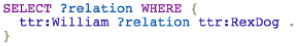
\includegraphics[width=150px]{img/sparqlRelation.png}
      \captionof{figure}{Antwort Frage 1}
      \label{fig:Antwort Frage 1}
\end{Figure}

\textit{Wessen Haustier ist Rex?}
\begin{Figure}
   \centering
   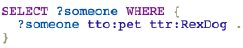
\includegraphics[width=150px]{img/sparqlOwnership.png}
      \captionof{figure}{Antwort Frage 2}
      \label{fig:Antwort Frage 2}
\end{Figure}

\textit{Welche Haustiere hat William?}
\begin{Figure}
   \centering
   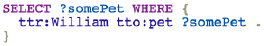
\includegraphics[width=150px]{img/sparqlPet.png}
      \captionof{figure}{Antwort Frage 3}
      \label{fig:Antwort Frage 3}
\end{Figure}

\chapter{Vorteile von eMedikation - L12 / L13}

\begin{itemize}
   \item \textbf{eMedication / ePrescription}
   \item Kontrollen im Bestell- und Verabreichungsprozess anhand von evidenzbasierten Richtlinien durchführen
   \item Administration durch Barcode und RFID Medikation
   \item Dosierungsanlage (Roboter)
   \item Verwendung und Interaktion der CIS Informationen (Laborresultate, Allergien etc.)
   \item Tracking der Medikation (Verwendung, Kosten und Abrechnung)
   \item \textbf{Electronic Medication Administration Record (eMar)}
   \item Bereitstellung eines langfristigen Verordnungsdatensatzes
   \item Überprüfung der Formalitäten, Compliance und Erstattungen
   \item Warnungen über Wechselwirkungen von Medikamenten
   \item Abwicklung über das Telefon für die Nachfüllung entfällt
   \item Lesefehler bei der Apotheke entfällt
   \item \textbf{Bar-Code-enabled Point of Core (BPOC)}
   \subitem Durch Barcode bei den Medikamenten und am Handgelenk des Patienten wird sichergestellt $\rightarrow$ korrekte/r Patient, Medikamentation, Dosierung, Zeit, Ablauf
   \subitem Alternative Verwendung durch RFID
\end{itemize}

\end{document}